\documentclass[tikz,border=6pt]{standalone}
% Shared style for the HERMESS schematic figures (compiled by build.sh).
% ETH palette; Latin Modern (the LaTeX default) to match the documentation.
\usepackage{amsmath}
\usepackage{tikz}
\usetikzlibrary{arrows.meta,positioning,calc,shapes.geometric,circuits.ee.IEC}
\definecolor{ethblue}{HTML}{215CAF}
\definecolor{ethpetrol}{HTML}{007894}
\definecolor{ethgrey}{HTML}{6F6F6F}
\tikzset{
  block/.style      = {draw=ethblue, thick, fill=ethblue!8, minimum height=9mm,
                       minimum width=16mm, inner sep=2.5pt, align=center},
  sum/.style        = {draw=ethblue, thick, circle, fill=white, minimum size=4.5mm, inner sep=0pt},
  sig/.style        = {-{Latex[length=2.4mm]}, thick},
  wire/.style       = {thick},
  node distance     = 9mm and 12mm,
  every node/.style = {font=\small},
  lbl/.style        = {font=\small, inner sep=1.5pt},
  port/.style       = {font=\small\itshape, text=ethgrey},
}

\usetikzlibrary{decorations.pathmorphing}
\begin{document}
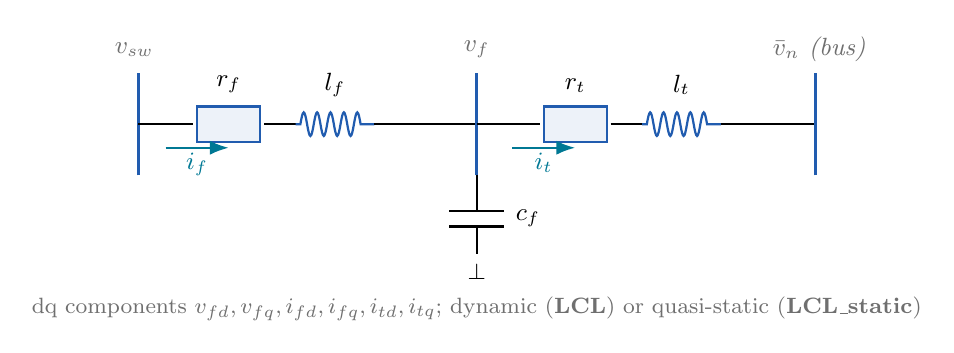
\begin{tikzpicture}[x=1cm,y=1cm,
  res/.style={draw=ethblue, thick, fill=ethblue!8, minimum width=8mm, minimum height=4.5mm, inner sep=1pt},
  coil/.style={thick, decorate, decoration={coil, aspect=0, segment length=1.7mm, amplitude=1.5mm, pre length=0.6mm, post length=0.6mm}}]
  % switching-voltage source node
  \draw[very thick, ethblue] (0,-0.3) -- (0,1.0);
  \node[port] at (-0.05,1.3) {$v_{sw}$};
  % converter-side branch r_f, l_f
  \draw[wire] (0,0.35) -- (0.7,0.35);
  \node[res] (rf) at (1.15,0.35) {};  \node[lbl, above=1mm of rf] {$r_f$};
  \draw[wire] (1.6,0.35) -- (2.0,0.35);
  \draw[coil, ethblue] (2.0,0.35) -- (3.0,0.35);  \node[lbl] at (2.5,0.85) {$l_f$};
  \draw[wire] (3.0,0.35) -- (4.3,0.35);
  \node[port] at (4.3,1.3) {$v_{f}$};
  \draw[very thick, ethblue] (4.3,-0.3) -- (4.3,1.0);
  % filter capacitor
  \draw[wire] (4.3,-0.3) -- (4.3,-0.75);
  \draw[thick] (3.95,-0.75) -- (4.65,-0.75);
  \draw[thick] (3.95,-0.95) -- (4.65,-0.95);
  \node[lbl] at (4.95,-0.85) {$c_f$};
  \draw[wire] (4.3,-0.95) -- (4.3,-1.3) node[below] {\footnotesize$\perp$};
  % grid-side branch r_t, l_t
  \draw[wire] (4.3,0.35) -- (5.1,0.35);
  \node[res] (rt) at (5.55,0.35) {};  \node[lbl, above=1mm of rt] {$r_t$};
  \draw[wire] (6.0,0.35) -- (6.4,0.35);
  \draw[coil, ethblue] (6.4,0.35) -- (7.4,0.35);  \node[lbl] at (6.9,0.85) {$l_t$};
  \draw[wire] (7.4,0.35) -- (8.6,0.35);
  \draw[very thick, ethblue] (8.6,-0.3) -- (8.6,1.0);
  \node[port] at (8.65,1.3) {$\bar v_{n}$ (bus)};
  % currents
  \draw[sig, ethpetrol] (0.35,0.05) -- (1.15,0.05) node[midway, below, lbl, text=ethpetrol] {$i_f$};
  \draw[sig, ethpetrol] (4.75,0.05) -- (5.55,0.05) node[midway, below, lbl, text=ethpetrol] {$i_t$};
  \node[lbl, text=ethgrey] at (4.3,-2.0)
    {\footnotesize dq components $v_{fd}, v_{fq}, i_{fd}, i_{fq}, i_{td}, i_{tq}$; dynamic (\textbf{LCL}) or quasi-static (\textbf{LCL\_static})};
\end{tikzpicture}
\end{document}
